\PassOptionsToPackage{unicode=true}{hyperref} % options for packages loaded elsewhere
\PassOptionsToPackage{hyphens}{url}
%
\documentclass[
]{book}
\usepackage{lmodern}
\usepackage{amssymb,amsmath}
\usepackage{ifxetex,ifluatex}
\ifnum 0\ifxetex 1\fi\ifluatex 1\fi=0 % if pdftex
  \usepackage[T1]{fontenc}
  \usepackage[utf8]{inputenc}
  \usepackage{textcomp} % provides euro and other symbols
\else % if luatex or xelatex
  \usepackage{unicode-math}
  \defaultfontfeatures{Scale=MatchLowercase}
  \defaultfontfeatures[\rmfamily]{Ligatures=TeX,Scale=1}
\fi
% use upquote if available, for straight quotes in verbatim environments
\IfFileExists{upquote.sty}{\usepackage{upquote}}{}
\IfFileExists{microtype.sty}{% use microtype if available
  \usepackage[]{microtype}
  \UseMicrotypeSet[protrusion]{basicmath} % disable protrusion for tt fonts
}{}
\makeatletter
\@ifundefined{KOMAClassName}{% if non-KOMA class
  \IfFileExists{parskip.sty}{%
    \usepackage{parskip}
  }{% else
    \setlength{\parindent}{0pt}
    \setlength{\parskip}{6pt plus 2pt minus 1pt}}
}{% if KOMA class
  \KOMAoptions{parskip=half}}
\makeatother
\usepackage{xcolor}
\IfFileExists{xurl.sty}{\usepackage{xurl}}{} % add URL line breaks if available
\IfFileExists{bookmark.sty}{\usepackage{bookmark}}{\usepackage{hyperref}}
\hypersetup{
  pdftitle={Test Doc},
  pdfauthor={Me},
  pdfborder={0 0 0},
  breaklinks=true}
\urlstyle{same}  % don't use monospace font for urls
\usepackage{longtable,booktabs}
% Allow footnotes in longtable head/foot
\IfFileExists{footnotehyper.sty}{\usepackage{footnotehyper}}{\usepackage{footnote}}
\makesavenoteenv{longtable}
\usepackage{graphicx,grffile}
\makeatletter
\def\maxwidth{\ifdim\Gin@nat@width>\linewidth\linewidth\else\Gin@nat@width\fi}
\def\maxheight{\ifdim\Gin@nat@height>\textheight\textheight\else\Gin@nat@height\fi}
\makeatother
% Scale images if necessary, so that they will not overflow the page
% margins by default, and it is still possible to overwrite the defaults
% using explicit options in \includegraphics[width, height, ...]{}
\setkeys{Gin}{width=\maxwidth,height=\maxheight,keepaspectratio}
\setlength{\emergencystretch}{3em}  % prevent overfull lines
\providecommand{\tightlist}{%
  \setlength{\itemsep}{0pt}\setlength{\parskip}{0pt}}
\setcounter{secnumdepth}{5}
% Redefines (sub)paragraphs to behave more like sections
\ifx\paragraph\undefined\else
  \let\oldparagraph\paragraph
  \renewcommand{\paragraph}[1]{\oldparagraph{#1}\mbox{}}
\fi
\ifx\subparagraph\undefined\else
  \let\oldsubparagraph\subparagraph
  \renewcommand{\subparagraph}[1]{\oldsubparagraph{#1}\mbox{}}
\fi

% set default figure placement to htbp
\makeatletter
\def\fps@figure{htbp}
\makeatother

\usepackage{booktabs}
\usepackage{longtable}
\usepackage{array}
\usepackage{multirow}
\usepackage{wrapfig}
\usepackage{float}
\usepackage{colortbl}
\usepackage{pdflscape}
\usepackage{tabu}
\usepackage{threeparttable}
\usepackage{threeparttablex}
\usepackage[normalem]{ulem}
\usepackage{makecell}
\usepackage{xcolor}

\title{Test Doc}
\author{Me}
\date{20 February 2020}

\begin{document}
\maketitle

{
\setcounter{tocdepth}{1}
\tableofcontents
}
\hypertarget{introduction}{%
\chapter*{Introduction}\label{introduction}}
\addcontentsline{toc}{chapter}{Introduction}

The purpose of this document is to collate the methods used to access, collect, process, and analyze derived data used to describe the status and trend of social, economical, ecological, and biological conditions

Trouble shooting the rnaturaleathhires issues in tech doc

\hypertarget{primary-production-required}{%
\chapter{Primary Production Required}\label{primary-production-required}}

\textbf{Description}: Time Series of Primary Production Required to sustain reported landings.

\textbf{Found in}: State of the Ecosystem - Gulf of Maine \& Georges Bank (2020+), State of the Ecosystem - Mid-Atlantic (2020+)

\textbf{Indicator category}: Database pull with analysis; Published methods

\textbf{Contributor(s)}: Michael Fogarty, Andrew Beet

\textbf{Data steward}: Andrew Beet, \href{mailto:andrew.beet@noaa.gov}{\nolinkurl{andrew.beet@noaa.gov}}

\textbf{Point of contact}: Andrew Beet, \href{mailto:andrew.beet@noaa.gov}{\nolinkurl{andrew.beet@noaa.gov}}

\textbf{Public availability statement}: Source data is not publicly availabe due to PII restrictions.

\hypertarget{methods}{%
\section{Methods}\label{methods}}

The index is a measure of the impact of fishing on the base of the foodweb. The amount of potential yield we can expect from a marine ecosystem depends on the amount of production entering at the base of the food web, primarily in the form of phytoplankton; the pathways this energy follows to reach harvested species; the efficiency of transfer of energy at each step in the food web; and the fraction of this production that is removed by the fisheries. Species such as scallops and clams primarily feed directly on larger phytoplankton species and therefore require only one step in the transfer of energy. The loss of energy at each step can exceed 80-90\%. For many fish species, as many as 2-4 steps may be necessary. Given the trophic level and the efficiency of energy transfer of the species in the ecosystem the amount phytoplankton production required (PPR) to account for the observed catch can be estimated.

The index for Primary Production Required (PPR) was adapted from (Pauly and Christensen \protect\hyperlink{ref-pauly1995ppr}{1995}).

\[PPR_t = \sum_{i=1}^{n_t}  \left(\frac{landings_{t,i}}{9}\right) \left(\frac{1}{TE}\right)^{TL_i-1}\]

where \(n_t\) = number of species in time \(t\), \(landings_{t,i}\) = landings of species \(i\) in time \(t\), \(TL_i\) is the trophic level of species \(i\), \(TE\) = Trophic efficiency. The PPR estimate assumes a 9:1 ratio for the conversion of wet weight to carbon and a 15\% transfer efficiency per trophic level, (\(TE\) = 0.15)

The index is presented as a percentage of \href{https://noaa-edab.github.io/tech-doc/chl-pp.html}{estimated primary production} (PP) available over the geographic region of interest, termed an \href{https://noaa-edab.github.io/tech-doc/comdat.html}{Ecological Production Unit} (EPU). The scaled index is estimated by dividing the PPR index in year \(t\) by the estimated primary production in time \(t\).

\[scaledPPR_t = \frac{PPR_t}{PP_t}\]

The species selected in each year were determined by their cumulative contribution to total landings. A threshold of at least 80\% of the total landings is used.

\hypertarget{data-sources}{%
\subsection{Data sources}\label{data-sources}}

Data for this index come from a variety of sources. The landings data come from the Commercial Fishery Database (CFDBS), species trophic level information come from \href{http://fishbase.de}{fishbase} and \href{http://sealifebase.ca}{sealifebase}, and primary production estimates are derived from \href{https://noaa-edab.github.io/tech-doc/chl-pp.html}{satellites}. Some of these data are typically not available to the public.

\hypertarget{data-extraction}{%
\subsection{Data extraction}\label{data-extraction}}

Landings are extracted from the commercial fisheries database (CFDBS) using the methods described in the chapter \href{https://noaa-edab.github.io/tech-doc/comdat.html}{Commercial Landings Data.}

Trophic level information for each species is obtained from \href{http://fishbase.de}{fishbase} and \href{http://sealifebase.ca}{sealifebase} using the R package \href{https://github.com/ropensci/rfishbase}{rfishbase} (Froese and Pauly \protect\hyperlink{ref-froese2019fishbase}{2019}) in tandem with the package \href{https://github.com/andybeet/indexPPR/}{indexPPR.}

Primary Production is estimated using the methods described in the chapter \href{https://noaa-edab.github.io/tech-doc/chl-pp.html}{Chlorophyll a and Primary Production.}

\hypertarget{data-analysis}{%
\subsection{Data analysis}\label{data-analysis}}

Annual (wet weight) landings are calculated for each species for a given EPU. For each year the landings are sorted in descending order by species and the cumulative landings are calculated. The top species that accounted for 80\% of total cumulative landings are selected. The trophic level for each of these species are then obtained from fishbase/sealifebase. At this point the PPR index is calculated. The units of the index
are \(gCyear^{-1}\) for the EPU. The index is converted to \(gCm^{-2}year^{-1}\) by dividing by the area (in \(m^2\)) of the EPU.

To normalize the index the total Primiary Production for the given EPU is required. This is calculated as described in the chapter \href{https://noaa-edab.github.io/tech-doc/chl-pp.html}{Chlorophyll a and Primary Production}. The units are also converted to \(gCm^{-2}year^{-1}\).

The index is then normalized by dividing the index in year t by the total primary production in time \(t\).

\hypertarget{plotting}{%
\subsection{Plotting}\label{plotting}}

Four plots are produced for each EPU:

\begin{itemize}
\tightlist
\item
  The normalized PPR index (along with the associated landings).
\item
  Total primary production
\item
  Mean trophic level of the species included in the index (weighted by their landings)
\item
  Species composition of landings
\end{itemize}

All created using the \href{https://github.com/andybeet/indexPPR}{indexPPR}

See the \href{https://github.com/andybeet/indexPPR/tree/master/vignettes}{workedExample vignette} in the \href{https://github.com/andybeet/indexPPR/}{indexPPR} package for plotting code.

\hypertarget{georges-bank-gb}{%
\subsubsection{Georges Bank (GB)}\label{georges-bank-gb}}

\hypertarget{gulf-of-maine-gom}{%
\subsubsection{Gulf of Maine (GOM)}\label{gulf-of-maine-gom}}

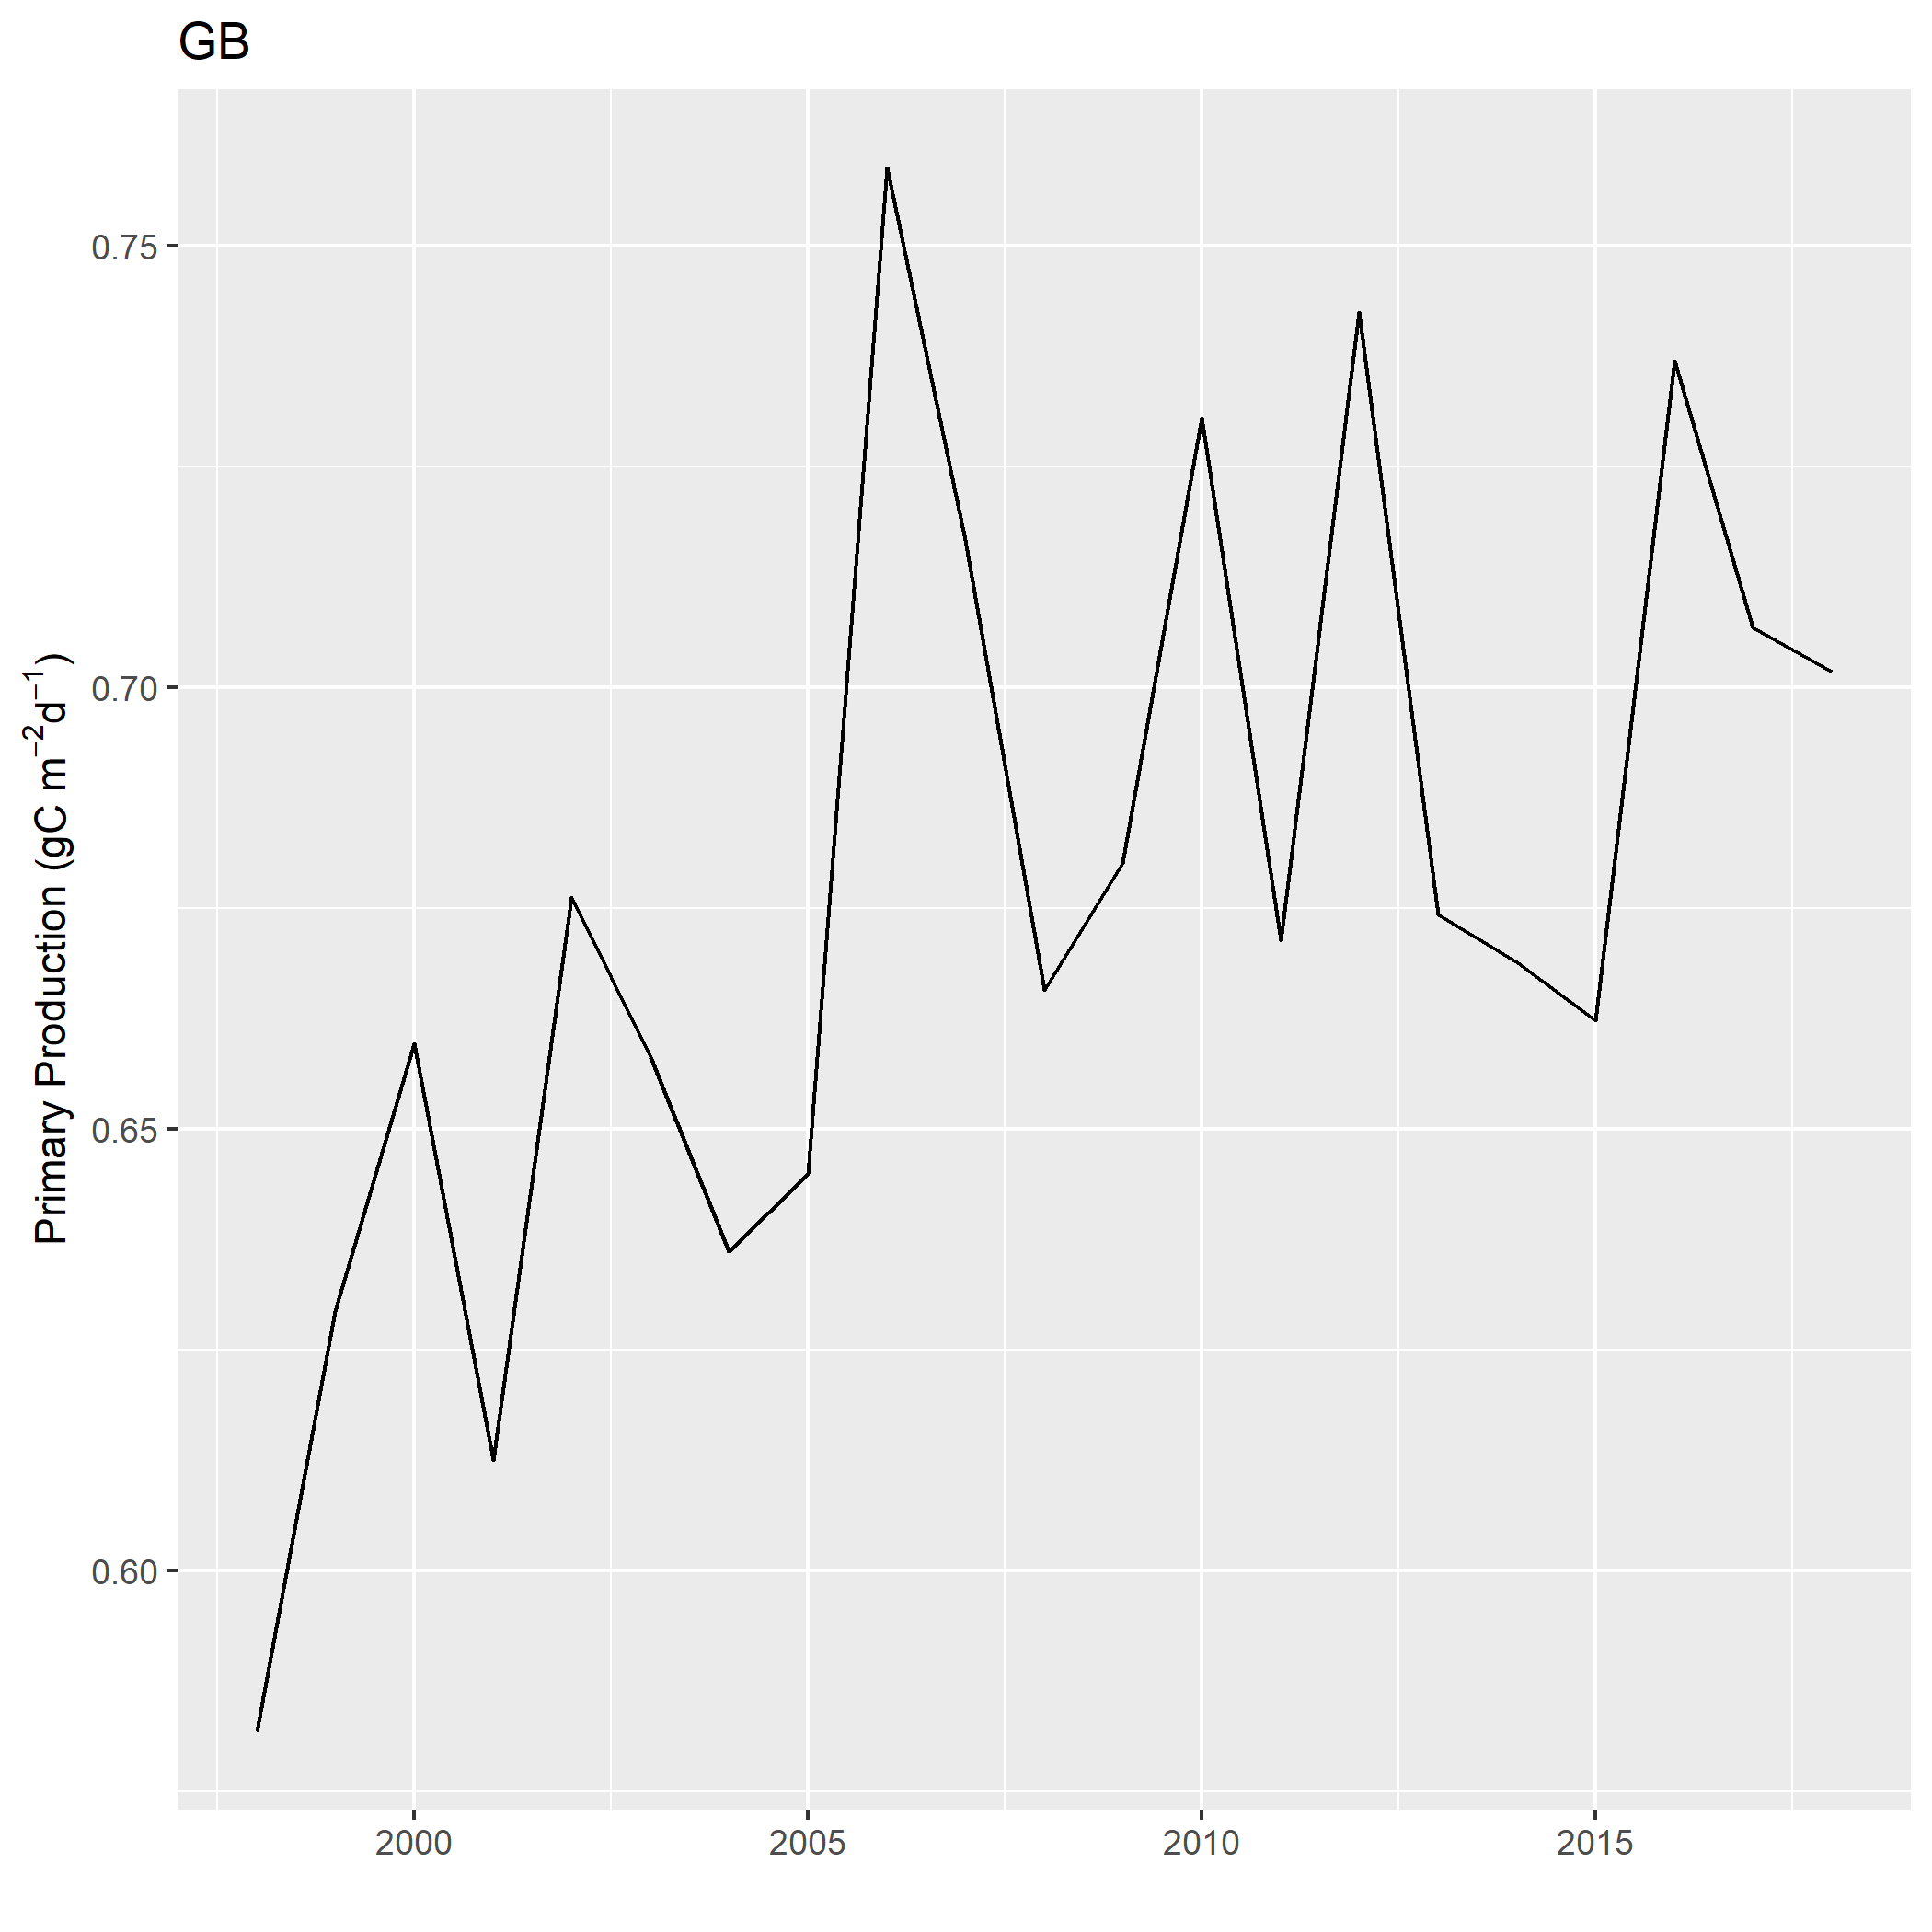
\includegraphics[width=0.5\linewidth]{/home/travis/build/bbest/test-doc/figures/test}

\hypertarget{mid-atlantic-bight-mab}{%
\subsubsection{Mid-Atlantic Bight (MAB)}\label{mid-atlantic-bight-mab}}

\hypertarget{references}{%
\chapter*{References}\label{references}}
\addcontentsline{toc}{chapter}{References}

\hypertarget{refs}{}
\leavevmode\hypertarget{ref-froese2019fishbase}{}%
Froese, R, and D Pauly, eds. 2019. \emph{Fishbase} (version 08/2019).

\leavevmode\hypertarget{ref-pauly1995ppr}{}%
Pauly, D, and V Christensen. 1995. ``Primary Production Required to Sustain Global Fisheries.'' \emph{Nature} 374: 255--57. \url{https://doi.org/https://doi.org/10.1038/374255a0}.

\end{document}
